\chapter{Ergebnisanalyse}

\todo{nochmal schauen ob Überleitung noch stimmt wenn Implementierungsteil geschrieben wurde...}
\todo{Verweis auf Anhang mit allen Tabellen für Metrikinformationen}

Nachdem im letzten Abschnitt ausführlich beschrieben wurde wie der komplette Komponentenstack im Detail implementiert wurde, werden im Folgenden auf die erhaltenen Metriken erläutert. Es wird insbesondere auf die Bedeutung einzelner Messwerte, sowie auf mögliche Begründungen dieser eingangen. Die genauen Messwerte wurden im Anhang aufgelistet und sind ebenfalls unter folgender Url einsehbar: \url{https://github.com/derMacon/serverless-bsc-thesis/tree/main/data} \todo{am Ende nochmal nachschauen ob URL weiterhin stimmt}


\todo{folgende Stichpunkte entfernen}
\begin{itemize}
  \item Latenzzeit im Durchschnitt sowie als zeitliche Historie
  \begin{itemize}
    \item Abschnitt \emph{vor} Datenaufnahme gesondert betrachten
    \item Abschnitt \emph{nach} Datenaufnahme gesondert betrachten
    \item Gesamte Pipeline betrachten
  \end{itemize}
  \item Skalierungsdauer jeweils pro verwendeter Backend-Technologie festzuhalten
  \begin{itemize}
    \item Skalierung anhand eingehender Nachrichten mittels Stufenmodell
    \item Skalierung mittels direkter Benutzeranfrage (ohne eingehende Nachrichten)
    \item Metriken als Datensätze in einer Datenbank hinterlegt
    \item Durchschnittliche Startzeit pro Containeranzahl 
    \item Durchschnittliche Startzeit pro Skalierungsstufe 
    \item Gesamtdurchschnittliche Startzeit als einzelner Messwert
    \item Metriken als zeitlicher visualisiert
  \end{itemize}
\end{itemize}


\section{Ergebnisse}
\begin{itemize}
  \item Vorstellung der erhaltenen Daten
  \item Interpretation / Analyse allerdings Teil vom naechsten Kapitel?
\end{itemize}

\subsection{Latenzzeit}
Die wichtigsten Messdaten bezüglich der Leistungsfähigkeit des Systems beziehen sich auf den Datendurchsatz beziehungsweise die entsprechende Latenzzeit. In der Tabelle \ref{tab:latency} wurden diese für die beiden betrachteten Backendtechnologien gegenübergestellt. Alle Angaben wurden in Millisekunden erfasst. Ein im System eingegangene Nachricht verweilt bei Bearbeitung durch einen Node.js Konsumenten im Schnitt 38 Sekunden, während sich dieser Wert bei Spring Boot auf über eine Minute beläuft. Diese Werte bilden lediglich einen Durchschnitt aller erhaltenen Metriken ab, eine genauere Aufteilung bezüglich des Zusammenhangs zu den Skalierungsgrößen erfolgt im nächsten Abschnitt (siehe \todo{Ref einfuegen}). Der Gesamtdurchschnitt setzt sich aus zwei Zeitangaben der Pipeline zusammen: 

\begin{enumerate}
  \item Den Nachrichteneingang: Diese Metrik beschreibt den Zeitraum zwischen erhaltener Anfrage im System und Acknowledgement durch die Konsumer-Komponente, dass die Nachricht nun bearbeitet wird. Sie beläuft sich bei der Node.js Komponente auf ungefähr 34 Sekunden und 58 Sekunden bei der Spring-Boot-Komponente. 
  \item Die Verarbeitungsdauer: Diese Metrik beschreibt den Zeitraum zwischen Acknowledgement durch den Konsumer, dass die Nachricht erhalten wurde, sowie dem Abspeichern des extrahierten Wertes durch den Konsumenten in der Datenbank. Dieser Werte beläuft sich bei beiden Implementierung auf etwas über drei Sekunden. Bei dieser Metrik liegt der Fokus allerdings auf dem minimalen Zeitunterschied im Millisekundenbereich, da in beide Implementierungen eine künstliche Verlangsamung (\emph{Sleep-Funktion}) eingebaut wurde um die erhaltenen Messwerte besser nachvollziehen zu können. Bei Node.js liegt die tatsächliche Verarbeitungsdauer bei 388 Millisekunden \emph{(total 3388)}, während sie bei Spring Boot bei 29 Millisekunden liegt \emph{(total 3029)}.
\end{enumerate}

\begin{wraptable}{r}{5.5cm}
	\centering
	\caption[Latenzzeit - Vergleich]{Latenzzeiten}
  \label{tab:latency}
  \hspace{1cm}
  \begin{tabular}{@{}lc@{}}
    \toprule
    Metrik & Dauer \\
    \midrule
    Node.js \\
    \hspace{3mm}Gesamtdurchschnitt & 38416 \\
    \hspace{3mm}Nachrichteneingang & 35027 \\
    \hspace{3mm}Verarbeitungsdauer & 3388 \\
    \midrule
    Spring Boot \\
    \hspace{3mm}Gesamtdurchschnitt & 61800 \\
    \hspace{3mm}Nachrichteneingang & 58771 \\
    \hspace{3mm}Verarbeitungsdauer & 3029 \\
    \bottomrule
  \end{tabular}
\end{wraptable} 


\subsection{Skalierungsdauer}
Diese Gruppe von Metriken bezieht sich auf die genauen Zeiträume, welche benötigt werden, um einen Container mit der entsprechenden Implementierung hochzufahren. Die ermittelten Zeiten stellen im Folgenden die durchschnittlichen Initialisierungszeiten eines einzelnen Containers dar. Sie beziehen sich nicht auf auf die Gesamtdauer der Initialisierungsphase aller beteiligten Container.

\paragraph{Aufschlüsselung nach Services}
Die abstrakteste Metrik bezieht sich auf den durchschnittlichen Zeitraum zum Initialisieren der Container eines bestimmten Services. Hierbei wird zwischen der Node.js sowie Spring-Boot-Komponente zum konsumieren der Eingangsnachrichten unterschieden. Die Container, welche eine Node.js Instanz beinhalten, benötigen im Schnitt 6.6 Sekunden zum Hochfahren, während diejenigen mit einer Spring-Instanz 35.3 Sekunden brauchen. Diese relativ großen Zeiträume lassen sich unter anderem auf die Anzahl der hochgefahrenen Instanzen zurückführen. Eine genauere Aufschlüsselung dieses Prozesses erfolgt in den nächsten Abschnitten. 


\begin{figure}
	\centering
	\begin{minipage}[b]{0.4\textwidth}
		\begin{tikzpicture}
			\begin{axis}[
					width  = 0.8\textwidth,
					height = 8cm,
					major x tick style = transparent,
					ybar=2*\pgflinewidth,
					bar width=14pt,
					ymajorgrids = true,
					xlabel = {Service},
					ylabel = {{\o} Initialisierungsgeschw.},
					symbolic x coords={Node.js,Spring Boot},
					xtick = data,
					scaled y ticks = false,
					enlarge x limits=0.25,
					ymin=0,
					legend cell align=left,
					legend style={
						at={(1,1.05)},
						anchor=south east,
						column sep=1ex
					}
				]
				\addplot[style={bblue,fill=bblue,mark=none}]
				coordinates {(Node.js,6.610) (Spring Boot,35.336)};
			\end{axis}
		\end{tikzpicture}
		\caption[Startzeit Container - Service]{Serviceübersicht}
		\label{fig:specContainers}
	\end{minipage}%
	\begin{minipage}[b]{0.6\textwidth}
		\begin{tikzpicture}
			\begin{axis}[
					width  = 0.9\textwidth,
					height = 8cm,
					major x tick style = transparent,
					ybar=2*\pgflinewidth,
					bar width=14pt,
					ymajorgrids = true,
					xlabel = {Skalierungsstufe},
					ylabel = {{\o} Initialisierungsgeschw.},
					symbolic x coords={Stufe1,Stufe2,Stufe3},
					xtick = data,
					scaled y ticks = false,
					enlarge x limits=0.25,
					ymin=0,
					legend cell align=left,
					legend style={
						at={(1,1.05)},
						anchor=south east,
						column sep=1ex
					}
				]
				\addplot[style={bblue,fill=bblue,mark=none}]
				coordinates {(Stufe1,2.976) (Stufe2,3.892) (Stufe3,6.898)};
				
				\addplot[style={ggreen,fill=ggreen,mark=none}]
				coordinates {(Stufe1,8.056) (Stufe2,16.019) (Stufe3,36.582)};
				
				\legend{Node.js,Spring Boot}
			\end{axis}
		\end{tikzpicture}
		\caption[Startzeit Container - Stufenweise]{Stufenübersicht}
		\label{fig:specContainers}
	\end{minipage}
\end{figure}


\paragraph{Aufschlüsselung nach Skalierungsstufe}
Um einen beispielhaften Skalierngsalgorithmus zu implementieren wurde ein Regelsatz verfasst welcher vom Alert-Manager zur Laufzeit automatisch in einem festgelegten Interval ausgewertet wird. Um diesen Regelsatz zu Vorführungszwecken nicht unnötig ausführlich zu gestalten, wurde das Hinzufügen neuer Instanzen in Stufen organisiert. 

Im durchgeführten Testszenario betrug die Grenze zum Überschreiten der ersten Stufe 15, für die zweite Stufe 30 und für die Dritte Stufe 100 unbeantwortete Nachrichten in der jeweiligen Warteschlange. Wenn im Folgenden von einem Burst gesprochen wird, ist hiermit das Überschreiten einer dieser Grenzen gemeint. Bei dem kleinst möglichen Burst bezüglich der Warteschlange der Node.js-Komponente, nimmt das System im Schnitt 2.9 Sekunden zum Starten der Container in Anspruch um der Arbeitslast nach Skalierung mit insgesamt 5 Containern zu begegnen. Bei der Spring-Boot-Komponente wurde hierfür ein Wert von 8 Sekunden gemessen. Im mittleren Grenz-Intervall wurde bezüglich Node.js eine Initialisierungsdauer von 3.8 Sekunden und auf Seiten von Spring 16 Sekunden festgestellt um nach der Skalierung mit 10 Instanzen zu arbeiten. Beim höchsten Burst werden kam es zu einer bei Node.js zu einer Initialisierungsphase von 6.9 Sekunden und bezüglich Spring zu 36.6 Sekunden. Hierbei sollen am Ende 30 Containerinstanzen des Konsumenten arbeitsbereit sein. Da beim Skalierungsalgorithmus mit den beschriebenen Stufen gearbeitet wird, kann hierbei nicht genau gesagt werden, wie viele Container genau im Endeffekt initialisiert wurden, da hierbei stets mit den Differenzen zwischen den Stufen gearbeitet wird. Wenn zum Beispiel bereits \emph{n} Container laufen wenn neue Nachrichten einen Burst verursachen, sollen nur die benötigten Instanzen kreiert werden, um genau die fehlende Anzahl zu decken. Die genaue Übersicht nach parallelen Instanziierungen wurde im Paragraphen (siehe Abschnitt \ref{par:specContainer}) genauer beschrieben.


\paragraph{Aufschlüsselung nach Containeranzahl}
\label{par:specContainer}
Die grundlegendste Metrik beschreibt die Zeiten aufgeschlüsselt nach Anzahl gleichzeitig hochfahrender Container (siehe \ref{fig:specContainers}). Wie im Graphen erkennbar, handelt es sich um ein lineares Wachstum. Mit jedem zusätzlichen Container, der zeitgleich erstellt werden soll, dauert der Initialisierungsprozess bei der Spring-Implementierung im Schnitt 1611 Millisekunden länger. Bei der Node Implementierung liegt dieser Wert bei 194 Millisekunden. So dauert das Initialisieren eines einzelnen neuen Containers bei der Spring-Boot-Komponente 4,8 Sekunden während sich dieser Wert bei der Node.js-Koponente lediglich 2,6 Sekunden beläuft. Um diese nach Containeranzahl aufgeschlüsselten Werte zu erhalten, wurde nicht wie bei den anderen Skalierungstests auf die öffentliche Schnittstelle mittels Nachrichtengenerierung zurückgegriffen, es wurde stattdessen eine interne Schnittstelle mittels dediziertem Skript verwendet um möglichst Störungsfrei direkt auf die Komponente welche das Skalieren orchestriert zuzugreifen. Die nachfolgenden Metriken wurden allerdings durch die öffentliche Schnittstelle generiert.

\begin{wrapfigure}{l}{0.55\textwidth}
  \centering
  \caption[Startzeit Container - Anzahl spezifisch]{Anzahlspezifisch}
  \label{fig:specContainers}
  \begin{tikzpicture}
    \begin{axis}[xlabel={Zusätzlich hochgefahrende Container}, ylabel={Startzeit}]
      \addplot table [x=additionalCnt, y=startupTime, col sep=comma] {kapitel/ergebnisanalyse/_data/springSpecificBenchmarks.csv};
      \addlegendentry{Spring Boot}
      \addplot table [x=additionalCnt, y=startupTime, col sep=comma] {kapitel/ergebnisanalyse/_data/nodeSpecificBenchmarks.csv};
      \addlegendentry{Node.js}
    \end{axis}
  \end{tikzpicture}
\end{wrapfigure}


\paragraph{Zeitliche Aufschlüsselung}
Wie in Bild \ref{fig:grafanaScreenshot01} zu sehen, wurde diverse Panels zur Zeitlichen Übersicht bereitgestellt. Diese wurden allerdings vor allem zu Kontrollzwecken implementiert. Diese visuelle Darstellung war während der Entwicklungszeit sehr hilfreich um Fehler frühzeitig zu erkennen und beheben zu können, für die Auswertung der Ergebnisse haben diese allerdings wenig Relevanz. Der Vollständigkeit halber soll an dieser Stelle dennoch eine kurze Zusammenfassung der zeitbasierten Messwerte erfolgen. Für alle bisher behandelten Metriken gibt es Panels im Grafana Dashboard. Da die zeitliche Erfassung in Grafana selbst allerdings intervallbasierte Abfragen stellt, sind diese im Vergleich zu den Werten, welche in der Datenbank durch das System selbst generiert und Abgelegt wurden, sehr ungenau. Selbstverständlich wurde in der bisherigen Analyse ausschließlich auf diese Daten zurückgegriffen. Bezüglich der Konsumenten wurde neben dem insgesamten durchschnittlichen Startverhalten auch der jeweils aktuelle Initialisierungszeitpunkt dargestellt. Hierbei war eine klare Korrelation zwischen der Anzahl der parallel startenden Konsumenten mit der Erhöhten Initialisierungsdauer zu beobachten. Außerdem wurden diverse Metriken aus dem Activemq selbst ausgelesen. So ist es zum Beispiel möglich nachzuvollziehen, wie viele Nachrichten sich zu einem gegebenen Zeitpunkt nicht nur in einer bestimmten Warteschlange sondern auch innerhalb des ganzen Systems befinden. Außerdem wurde die zeitliche Abfolge zwischen einem Burst an unbeantworteten Nachrichten und dem Anstieg der Containerinstanzen in einem Dashboard-Panel dargestellt.

\begin{figure}[ht!]
	\centering
	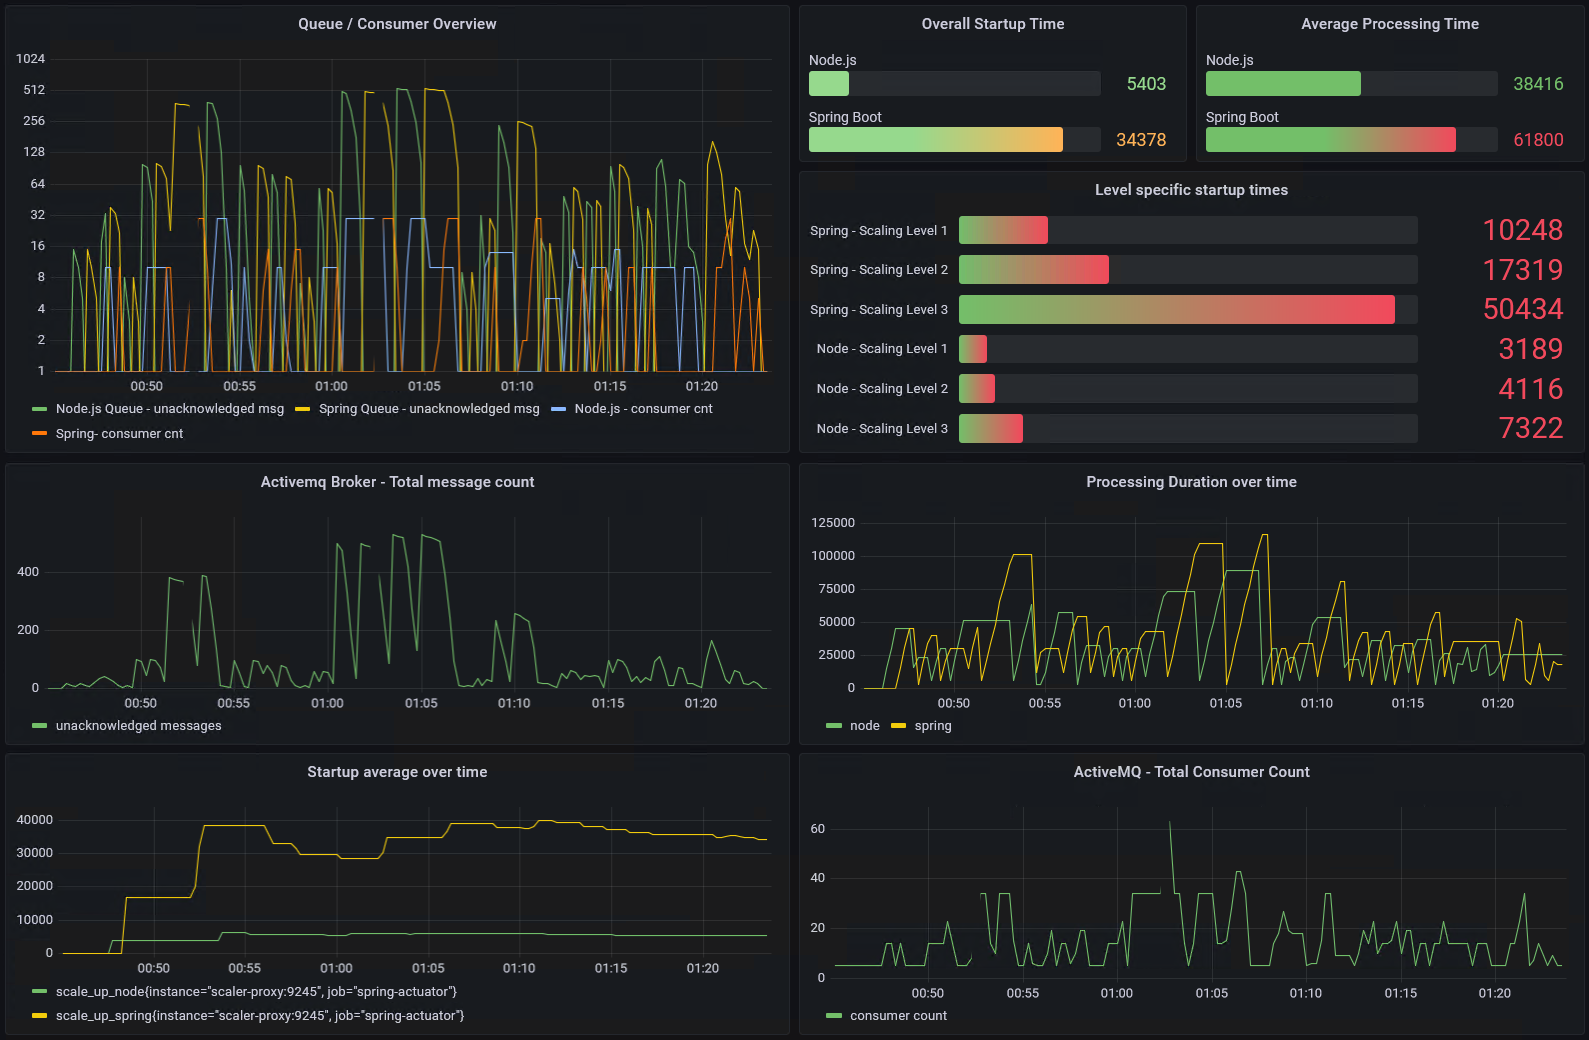
\includegraphics[width=\linewidth]{kapitel/problemloesung/implementierung/_img/grafana-dashboard-01}
	\caption[]{Grafana Dashboard}
	\label{fig:grafanaScreenshot01}
\end{figure}


\section{Analyse}
\begin{itemize}
  \item Interpretation / Analyse der Daten
  \item Begruendung fuer Verhalten suchen
\end{itemize}

\subsection{Latenzzeit}
Hinsichtlich der Latenzzeit überrascht vorallem die deutliche Diskrepanz zwischen der Initialisierungsdauer der unterschiedlichen Technologien. Durch die Unterteilung der Pipeline in die zwei Messwerte ist erkennbar, dass diese auf die zeitliche Dauer bis zum Nachrichteneingang zurückzuführen ist. Hierbei läuft die Dauer der Initialisierungsphasen weit auseinander (siehe \ref{ss:skalierungsdauer}).

Bezüglich der Verarbeitungsgeschwindigkeit ist die Spring-Boot Komponente jedoch im Vergleich schneller. Dies ist auf die Natur einer kompilierten Sprache zurückzuführen. Java Code wird im Vorwege in entsprechenden Bytecode übersetzt, während eine Skriptsprache wie Javascript innerhalb der Node.js-Komponente zur Laufzeit übersetzt wird. Da in den Komponenten nur minimale Logik verbaut wurde, ist der festgestellte zeitliche Unterschied in der Bearbeitungsdauer mit 359  Millisekunden zwar nicht so gravierend wie der Unterschied hinsichtlich der Initialisierungsphase der Container, allerdings drastischer als vorher angenommen. Da der Prototyp eine sehr einfache Ausführungslogik implementiert, ist dieser Messwert doch relativ hoch. In Anbetracht der Komplexität der realen Banking-Anwendung gilt es ein spezifisches Konzept für das Regelwerk zum Starten der Container zu entwerfen. Hierbei muss eine Untersuchung bezüglich der Rentabilität eines neuen startenden Containers gegenüber eines laufenden Containers evaluiert werden.


\subsection{Skalierungsdauer}
\label{ss:skalierungsdauer}
Die erheblich abweichende Initialisierungsgeschwindigkeit der beiden unterschiedlichen Komponenten lässt sich im Kern auf auf die Initialisierungs des Spring-Containers sowie des dazugehörgien Application-Contexts zurückführen. Das Framework bietet durch die ... \todo{Weiterschreiben, schauen ob es diese Erklärung schon irgendwo in der Thesis gibt.}
Kern des Spring Frameworks ist der \emph{Spring Container}. Dieser verwaltet fachliche und nichtfachliche Objekte, die eine Anwendung ausmachen. Die verwalteten Objekte werden als \emph{Beans} bezeichnet. "Eine Bean ist ein Objekt, das vom Spring-Container instanziiert und konfiguriert wurde und dessen Lebenszyklus vom Container verwaltet wird. Die Abhängigkeiten zwischen Beans sind als Metadaten im Container verfügbar" \cite[Kapitel~3.1.1]{simons-spring}. 


\section{Diskussion}

\subsection{Begr\"undung Startupzeit}
\begin{itemize}
  \item Warum Node.js schneller ist
\end{itemize}

\begin{itemize}
  \item Erlaeutern warum die erhaltenen Ergebnisse in einem real-life Szenario vielleicht nicht aussagekraeftig sein koennten
\end{itemize}
